\documentclass[t, screen, aspectratio=43]{beamer}
\usepackage[T1]{fontenc}
\usepackage[utf8]{inputenc}
\usepackage{epsf}
\usepackage{graphicx}
\usepackage{geometry}
\usepackage{tabularx}
\usepackage[table]{colortbl}
\usepackage{xcolor}
\usepackage{soul}
\usepackage[normalem]{ulem}
\usepackage{tikz}
\usepackage{subcaption}
\usepackage{hyperref}
\usepackage{color,soul}
\usepackage{skak}
% Use the NTNU-temaet for beamer 
% \usetheme[style=ntnu|simple|vertical|horizontal, 
%     language=bm|nn|en, 
%     smalltitle, 
%     city=all|trondheim|alesund|gjovik]{ntnu2017}
\usetheme[style=helvet,language=en]{ntnu2017}

\usepackage[english]{babel}
\usepackage[style=numeric,backend=biber,natbib=false,sorting=none]{biblatex}

\title[Short title]{Ultra low power integer-N ADPLL}
\subtitle{Master's thesis project - meeting 8}
\author[C Nielsen]{Cole Nielsen}
\institute[NTNU]{Department of Electronic Systems, NTNU}
\date{5 March 2020  (calendar week 10)}
%\date{} % To have an empty date

\addbibresource{example.bib} % Add bibliography database

% Set the reference style to numeric.
% See here: http://tex.stackexchange.com/questions/68080/beamer-bibliography-icon
\setbeamertemplate{bibliography item}[text] 

% Set bibliography fonts to a small size.
\renewcommand*{\bibfont}{\footnotesize}

\usepackage{tikz}
\usepackage{enumitem}
\newcommand*\mycirc[1]{%
\begin{tikzpicture}[baseline=(C.base)]
	\node[draw,circle,inner sep=1pt,minimum size=3ex](C){#1};
\end{tikzpicture}}


\begin{document}

\begin{frame}
	\titlepage%
\end{frame}

% Alternatively, special title page command to get a different background
% \ntnutitlepage

% #############################################################################
% This week
% #############################################################################

\begin{frame}
	\frametitle{Overview}
	\begin{block}{For this week...}
		\begin{enumerate}[itemsep=4pt,label=\protect\mycirc{\arabic*}]
			\scriptsize
			\item Some ring oscillator theory
			\item Oscillator topologies tested
			\item Final topology.
			\item Buffer/new BBPD topology
		\end{enumerate} 
	\end{block}	
\end{frame}


% #############################################################################
% This week
% #############################################################################


% #############################################################################
% Physical limits
% #############################################################################



% \begin{frame}
% 	\frametitle{Topology}
% 	\begin{block}{Ring oscillator.}
% 		\begin{minipage}{4cm}
% 			\vspace{1em}
% 			\tiny

% 			% \vspace{100em}
% 			\begin{itemize}[itemsep=4pt,label=\protect---]
% 				\item Can build ring oscillator with:
% 				\begin{itemize}[itemsep=4pt,label=$\bullet$]
% 					\item Linear stages
% 					\item Saturating stages
% 				\end{itemize}
% 			\end{itemize}
% 			\textbf{Linear}
% 			\begin{itemize}[itemsep=4pt,label=\protect---]
% 				\item Requires resistive load, tail current source for differential operation.
% 				\item Current biasing introduces correlated noise in every stage.
% 				\item Lower amplitude = lower SNR.
% 			\end{itemize}
% 			\textbf{Saturating}
% 			\begin{itemize}[itemsep=4pt,label=\protect---]
% 				\item Do not need current starvation, thus no correlated noise component.
% 				\item Larger swing = higher SNR
% 				\item According to [1], hard switching is the best option to improve phase noise.
% 			\end{itemize}
% 			% \vspace{-3em}
% 		\end{minipage}%
% 		% \hspace{-0.5cm}
% 		\begin{minipage}{8cm}
% 			\begin{figure}[htb!]
% 			        \centering
% 			        \includegraphics[width=0.8\textwidth, angle=0]{ro_pn_vs_length2}
% 			    % \caption{Approximate model for ring oscillator inverter delay cell.}
% 			\end{figure}
% 		\end{minipage}%

% 	\end{block}	
% \end{frame}

\begin{frame}
	\frametitle{Ring oscillator phase noise}
	\begin{block}{Channel length}
		\begin{minipage}{4cm}
			\vspace{1em}
			\tiny

			% \vspace{100em}
			\begin{itemize}[itemsep=4pt,label=\protect---]
				\item Simulated 5 stage ring oscillator.
				\item RVT devices, W/L = 5.
				\item Ran pss/pnoise.
				\item Computed FOM vs channel length (lower is better):
			\end{itemize}
				\begin{equation}
					\textnormal{FOM} = 10\log_{10}\left( \left( \frac{\Delta f}{f_0} \right)^2 \cdot\frac{\textnormal{P}_{total}}{\textnormal{1 mW}} \right)\hspace{1em} \textnormal{[dB]}
				\end{equation}
			\begin{itemize}[itemsep=4pt,label=\protect---]
				\item It is seen that FOM improves asymptotically to $\sim$ -165 with longer L.
				\item FOM < -160 dB $\rightarrow$ L $\geq$ 100 nm.
				\item L should be set as long as possible, while mantaining appropriate speed.
				\begin{itemize}[itemsep=4pt,label=$\bullet$]
					\item This is actually recommended in Razavi's new book.
				\end{itemize}
			\end{itemize}
			% \vspace{-3em}
		\end{minipage}%
		% \hspace{-0.5cm}
		\begin{minipage}{8cm}
			\begin{figure}[htb!]
			        \centering
			        \includegraphics[width=0.8\textwidth, angle=0]{ro_pn_vs_length2}
			    % \caption{Approximate model for ring oscillator inverter delay cell.}
			\end{figure}
		\end{minipage}%

	\end{block}	
\end{frame}

\begin{frame}
	\frametitle{Ring oscillator phase noise}
	\begin{block}{Theoretical limit applied}
		\scriptsize
		Ring oscillator phase noise limit from "Minimum Achievable Phase Noise of RC Oscillators", Navid et al. 2005:
		\begin{equation}
			PN_{min}(\Delta f)= 10\log 10\left(\frac{7.33k_BT}{P}\left(\frac{f_0}{\Delta f}\right)^2\right)
		\end{equation}
		\vspace{-.8em}\\
		If $f_0$ = 2.4 GHz, P = 50 $\mu$W, $\Delta f$= 1 MHz, T = 293 K, $\rightarrow$ \textbf{PN$_{min}$ = -84.7 dBc/Hz} \\
		-- This limit applied to the below FOM comparison (FOM PN=165 dB):
		\vspace{-1.5em}
		\center\includegraphics[width=0.75\textwidth, angle=0]{ro_perf.pdf}
	\end{block}
\end{frame}


\begin{frame}
	\frametitle{Ring oscillator model}
	\begin{block}{Assumptions.}
		\begin{minipage}{4cm}
			\vspace{1em}
			\tiny
		\begin{itemize}[itemsep=4pt,label=\protect---]
			\tiny
			\item Inverters modeled with ideal switches and lumped R and C components. R = $\langle g_{ch}\rangle^{-1}$, where $\langle g_{ch}\rangle$ is the average channel conductance during the propagation period $t_{pd}$
			\item Square law is valid ($L>>L_{min}$).
			\item In saturation during period of propagtion delay. Requires that 0.25$\cdot V_{DD}$ < $V_{th}$ < 0.5$\cdot V_{DD}$.
		\end{itemize}    
			% \vspace{100em}

			% \vspace{-3em}
		\end{minipage}%
		% \hspace{-0.5cm}
		\begin{minipage}{8cm}
			\begin{figure}[htb!]
			        \centering
			        \center\includegraphics[width=1\linewidth]{ro_model_fig.png}
			    % \caption{Approximate model for ring oscillator inverter delay cell.}
			\end{figure}
		\end{minipage}%

	\end{block}	
\end{frame}

\begin{frame}
	\frametitle{Ring oscillator model}
	\begin{block}{Ring oscillator model - equations 1}
			%\center\includegraphics[width=0.8\textwidth, angle=0]{loop_bandwidth.pdf}
	\scriptsize
	% \vspace{-1em}
		\tiny
		\textbf{Define current and voltage exponentials for active device}
		\begin{equation}
			I_{out}(t) = \frac{k_n}{2}\left(\frac{W}{L}\right)_n\left[\left(V_{in}(t) - V_t\right)^2 \right]  - I_{short} = \frac{k_n}{2}\left(\frac{W}{L}\right)_n\left[\left(V_{DD}\left(1-e^{-t/\tau}\right) - V_t\right)^2 - \left(\frac{V_{DD}}{2} -V_t\right)^2\right]
		\end{equation}
		\begin{equation}
			V_{out} = V_{DD}e^{-(t-t_{pd})/\tau}
		\end{equation}
		\tiny
		\textbf{Compute average transconductance}
		\begin{equation}
			\langle g_{ch} \rangle = \frac{1}{t_{pd}} \int_0^{t_{pd}}\frac{I_{out}(t)}{V_{out}(t)}dt
		\end{equation}
		\begin{equation}
			\langle g_{ch} \rangle = \frac{1}{2}\mu_nC_{ox}\left(\frac{W}{L}\right)_n\left[V_{DD}\left(\frac{7}{8\ln2}-1\right)-V_t\left(\frac{1}{\ln2}-1\right) \right]
		\end{equation}
		\textbf{Define node capacitance}
		\begin{equation}
			C = C_{ox}\left ( W_N L_N + W_P L_N \right) + C_L
		\end{equation}
		\textbf{Define oscillator frequency}
		\begin{equation}
			f_{osc}^{-1} = 2Nt_{pd} = \frac{2\ln(2)NC}{\langle g_{ch}\rangle}
		\end{equation}
	\end{block}
\end{frame}


\begin{frame}
	\frametitle{Ring oscillator model}
	\begin{block}{Unequal $V_t$ for NMOS and PMOS}
			%\center\includegraphics[width=0.8\textwidth, angle=0]{loop_bandwidth.pdf}
	\scriptsize
	% \vspace{-1em}
		\tiny
		\textbf{In the case of different threshold voltages for NMOS and PMOS:}
			\begin{equation}
				f_{osc}^{-1} = N(t_{pdn} + t_{pdp}) = \ln(2)NC\left(\frac{1}{\langle g_{ch}\rangle_n} + \frac{1}{\langle g_{ch}\rangle_p}\right) = \frac{2\ln(2)NC}{\langle g_{ch}\rangle'}
			\end{equation}	
			\textbf{Enforcing $\mu_nC_{ox}\left(\frac{W}{L}\right)_n = \mu_pC_{ox}\left(\frac{W}{L}\right)_p$ results in:}
			\begin{align}
				\langle g_{ch}\rangle' = \frac{1}{2}\mu_nC_{ox}\left(\frac{W}{L}\right)_n\frac{2 \alpha_n\alpha_p}{\alpha_n + \alpha_p} = \frac{1}{2}\mu_nC_{ox}\left(\frac{W}{L}\right)_n \alpha'
			\end{align}	
			\textbf{Thus $\alpha_n$ and $\alpha_p$ are found for the according threshold voltages and then $\langle g_{ch}\rangle$ can be found.}
			\begin{align}
				\alpha' =  \frac{2 \alpha_n\alpha_p}{\alpha_n + \alpha_p}, \hspace{1em} \alpha_x = \left[V_{DD}\left(\frac{7}{8\ln2}-1\right)-V_{tx}\left(\frac{1}{\ln2}-1\right) \right]
			\end{align}
	\end{block}
\end{frame}

\begin{frame}
	\frametitle{Ring oscillator model}
	\begin{block}{Frequency and power.}
			%\center\includegraphics[width=0.8\textwidth, angle=0]{loop_bandwidth.pdf}
	\scriptsize
	% \vspace{-1em}
		\tiny
		\textbf{Solving for oscillator frequency:}
			\begin{equation}
				f_{osc} = \frac{\mu_nC_{ox}}{4\ln2NC}\left(\frac{W}{L}\right)_n\left[V_{DD}\left(\frac{7}{8\ln2}-1\right)-V_t\left(\frac{1}{\ln2}-1\right) \right]
			\end{equation}
			\textbf{If capacitance is strictly proportional to gate area, and PMOS/NMOS are equal sized $C=2WLC_{ox}$:}
			\begin{equation}
				f_{osc} = \frac{\mu_n}{8\ln2N}\cdot\frac{1}{L^2}\left[V_{DD}\left(\frac{7}{8\ln2}-1\right)-V_t\left(\frac{1}{\ln2}-1\right) \right]
			\end{equation}
			\textbf{Power is $P = fC_{\Sigma}V_{DD}^2$, where $C_{\Sigma}$ is the total active capacitance. Thus:}
			\begin{equation}
				P_{osc} = Nf_{osc}CV_{DD}^2 = \frac{\mu_nC_{ox}}{4\ln2}\left(\frac{W}{L}\right)_n\left[V_{DD}\left(\frac{7}{8\ln2}-1\right)-V_t\left(\frac{1}{\ln2}-1\right) \right]
			\end{equation}
			\textbf{\color{red}It should be noted that the power consumption is proportional to FET aspect ratio (W/L).}
	\end{block}
\end{frame}

\begin{frame}
	\frametitle{Ring oscillator model}
	\begin{block}{Back gate tuning}
			%\center\includegraphics[width=0.8\textwidth, angle=0]{loop_bandwidth.pdf}
	\scriptsize
	% \vspace{-1em}
		\tiny
		\textbf{In FDSOI, the body effected is manifested as:}
		\begin{equation}
			V_t = V_{t0} - \gamma V_{BG}
		\end{equation}
		\textbf{Using this in the ring oscillator frequency equation, if $\gamma_n \approx \gamma_p$ and $V_{t0n}\approx V_{t0p}$:}
		\begin{equation}
			f_{osc} = \frac{\mu_nC_{ox}}{4\ln2NC}\left(\frac{W}{L}\right)_n\left[V_{DD}\left(\frac{7}{8\ln2}-1\right)-V_{t0}\left(\frac{1}{\ln2}-1\right) + \gamma V_{BG}\left(\frac{1}{\ln2}-1\right) \right]
		\end{equation}
		\textbf{Equivalently, defining $f_{osc} = f_{0,osc} + \Delta f_{osc}(V_{BG})$, where:}
		\begin{equation}
			\Delta f_{osc}(V_{BG}) = \gamma V_{BG}\frac{\mu_nC_{ox}}{4\ln2NC}\left(\frac{W}{L}\right)_n\left[\frac{1}{\ln2}-1\right]
		\end{equation}	
	\end{block}
\end{frame}

\begin{frame}
	\frametitle{Ring oscillator model}
	\begin{block}{Ring oscillator model - equations 3}
			%\center\includegraphics[width=0.8\textwidth, angle=0]{loop_bandwidth.pdf}
	\scriptsize
	% \vspace{-1em}
		\tiny
		\textbf{Constraining backgate voltage to [0, $V_{DD}$], the center frequency $f_c$ in the tuning range of the oscillator are then:}
		\begin{equation}
			f_{c} = \frac{\mu_nC_{ox}}{4\ln2NC}\left(\frac{W}{L}\right)_n\left[V_{DD}\left(\frac{7}{8\ln2}-1+\frac{\gamma}{2\ln2}-\frac{\gamma}{2}\right)-V_{t0}\left(\frac{1}{\ln2}-1\right)\right]
		\end{equation}
		\begin{equation}
			\Delta f = \gamma V_{DD}\frac{\mu_nC_{ox}}{4\ln2NC}\left(\frac{W}{L}\right)_n\left[\frac{1}{\ln2}-1\right]
		\end{equation}
		\textbf{The fractional tuning range of the oscillator is:}
		\begin{equation}
			\frac{\Delta f}{f_c} = \frac{\gamma V_{DD}\left( 1-\ln2 \right)}{V_{DD}\left(\frac{7}{8}-\ln2+\frac{\gamma}{2}-\frac{\gamma}{2}\ln2\right)-V_{t0}\left(1-\ln2\right)}
		\end{equation}	
		\textbf{If a N-bit DAC is used to control the oscillator, the resulting DCO gain is therefore:}
		\begin{equation}
			K_{DCO} = \frac{f_c}{2^{N_{DAC}}}\cdot\frac{\gamma V_{DD}\left( 1-\ln2 \right)}{V_{DD}\left(\frac{7}{8}-\ln2+\frac{\gamma}{2}-\frac{\gamma}{2}\ln2\right)-V_{t0}\left(1-\ln2\right)}
		\end{equation}	
		\textbf{$V_{t0}$ = 0.3V, $V_{DD}$=0.8, $\gamma$ = 0.07 yields 27.7\% tuning range. 	I need ca 0.5\%. Higher $V_{DD}$ = smaller $\frac{\Delta f}{f_c}$.}
	\end{block}
\end{frame}




\begin{frame}
	\frametitle{Good oscillator characteristics}
	\begin{block}{Hajimiri's phase noise theory}
		\begin{minipage}{6cm}
			\vspace{1em}
			\tiny

			% \vspace{100em}
			\begin{itemize}[itemsep=4pt,label=\protect---]
				\item Hajimiri's famous paper [2] introduces the concept of the impulse sensitivity function (ISF).
				\begin{figure}[htb!]
				        \centering
				        \includegraphics[width=0.5\textwidth, angle=0]{isf_func}
				    % \caption{Approximate model for ring oscillator inverter delay cell.}
				\end{figure}
				\item ISF defines phase shift of oscillator with unit impulse applied to different parts of the oscillator cycle.
				\item Transition periods most sensitive to noise.
				\item Differing rise/fall time results in net DC component in ISF
				\begin{itemize}[itemsep=4pt,label=$\bullet$]
					\item This increases oscillator noise susceptibility.
				\end{itemize}
				\item \textbf{\color{red}Good rise/fall symmetry required in design}.
			\end{itemize}

			% \vspace{-3em}
		\end{minipage}%
		% \hspace{-0.5cm}
		\begin{minipage}{6cm}
			\begin{figure}[htb!]
			        \centering
			        \includegraphics[width=0.7\textwidth, angle=0]{isf}
			    % \caption{Approximate model for ring oscillator inverter delay cell.}
			\end{figure}
		\end{minipage}%

	\end{block}	
\end{frame}


\begin{frame}
	\frametitle{Implementation}
	\begin{block}{Parallel topology}
		\begin{minipage}{6cm}
			\vspace{1em}
			\tiny

			\begin{itemize}[itemsep=4pt,label=\protect---]
				\item Utilize pseudo-differential inverter stage [3], in parallel with back gate tuned inverter.
				\begin{itemize}[itemsep=4pt,label=$\bullet$]
					\item Pseudo-differential stage couples oscillators, forcing crossing voltage $V_{DD}/2$.
					\item Back gate tuned oscillator used to adjust frequency.
				\end{itemize}			
				\item Ratioing the sizes two types of inverters can be used to adjust the VCO gain. A ratio of 1:1 should reduce the $K_{VCO}$ in half from what is expected from theory, a ratio of 3:1 (with pseudo-diff inverters being larger) will reduce $K_{VCO}$ by 4. 
				\item \textbf{Requires complementary control of backgate voltage for tuning.}
				\item \textbf{\color{red}Allows for 0-$V_{DD}$ control range.	}
			\end{itemize}
			% \vspace{-3em}
		\end{minipage}%
		% \hspace{-0.5cm}
		\begin{minipage}{6cm}
			\begin{figure}[htb!]
			        \centering
			        \includegraphics[width=0.8\textwidth, angle=0]{parallel_delay_cell}
			    % \caption{Approximate model for ring oscillator inverter delay cell.}
			\end{figure}
		\end{minipage}%

	\end{block}	
\end{frame}

\begin{frame}
	\frametitle{Implementation}
	\begin{block}{Device selection}
		\vspace{1em}
		\begin{minipage}{6cm}
			\tiny

			\begin{itemize}[itemsep=4pt,label=\protect---]
				\item Must use devices in N well (PFET, HVTPFET, SLVTNFET, LVTNFET) to not forward bias substrate diode.
				\item To achieve $V_{m}$ =  $V_{DD}/2$, PFET + LVTNFET give most reasonable W$_P$/W$_N$, ca 1.2-1.4.
				\begin{itemize}[itemsep=4pt,label=$\bullet$]
					\item SLVTNFET + PFET needs W$_P$/W$_N$ $\approx$ 8.
				\end{itemize}
			\end{itemize}
			% \vspace{-3em}
		\end{minipage}%
		% \hspace{-0.5cm}
		\begin{minipage}{6cm}
			\begin{figure}[htb!]
			        \centering
			        \includegraphics[width=0.8\textwidth, angle=0]{wp_pfet_lvtnfet_inv}
			    % \caption{Approximate model for ring oscillator inverter delay cell.}
			\end{figure}

		\end{minipage}%

	\end{block}	

\end{frame}

\begin{frame}
	\frametitle{Implementation}
	\begin{block}{Simulation}
		\begin{minipage}{6cm}
			\vspace{1em}
			\tiny

			\begin{itemize}[itemsep=4pt,label=\protect---]
				\item Good symmetry of rise time observed, with $V_{cm}$ close to $V_{DD}/2$ over the full oscillation cycle.
				\item \textbf{Observed 10.3\% fractional frequency tuning with L=150nm, FOM=-161 dB, 1:1 ratio of inverters.}
				\item I require $<$ 1\% fractional tuning range to achieve my $K_{DCO}$ with a 10b DAC, this will not work. The (W/L) becomes large to achieve a high inverter ratio, thus increases power too much.
			\end{itemize}
			% \vspace{-3em}
		\end{minipage}%
		% \hspace{-0.5cm}
		\begin{minipage}{6cm}
			\tiny
			\hspace{1em}\color{red}\textbf{Single ended outputs:}
			\vspace{-1em}
			\begin{figure}[htb!]
			        \centering
			        \includegraphics[width=0.7\textwidth, angle=0]{parallel_osc_wfm}
			    % \caption{Approximate model for ring oscillator inverter delay cell.}
			\end{figure}
			\vspace{-1em}
			\hspace{1em}\textbf{Common mode voltage:}
			\vspace{-1em}
			\begin{figure}[htb!]
			        \centering
			        \includegraphics[width=0.7\textwidth, angle=0]{parallel_cmv}
			    % \caption{Approximate model for ring oscillator inverter delay cell.}
			\end{figure}

		\end{minipage}%

	\end{block}	

\end{frame}


\begin{frame}
	\frametitle{Implementation}
	\begin{block}{Telescopic topology}
		\begin{minipage}{6cm}
			\vspace{1em}
			\tiny

			\begin{itemize}[itemsep=4pt,label=\protect---]
				\item Modify the pseudo-differential cell to have header/footer transistors with back gate control.
				\begin{itemize}[itemsep=4pt,label=$\bullet$]
					\item Cross-coupled devices force differential operation
					\item Header/footer devices used to adjust frequency.
				\end{itemize}				
				\item Ratioing the size of the header/footer devices to the size of the cross-coupling devices tunes $K_{VCO}$
				\item \textbf{Requires complementary control of backgate voltage for tuning.}
			\end{itemize}
			% \vspace{-3em}
		\end{minipage}%
		% \hspace{-0.5cm}
		\begin{minipage}{6cm}
			\begin{figure}[htb!]
			        \centering
			        \includegraphics[width=0.58\textwidth, angle=0]{tele_delay_cell}
			    % \caption{Approximate model for ring oscillator inverter delay cell.}
			\end{figure}
		\end{minipage}%

	\end{block}	
\end{frame}


\begin{frame}
	\frametitle{Implementation}
	\begin{block}{Telescopic design - simulation}
				\vspace{2em}
		\begin{minipage}{6cm}
			\tiny


			\begin{itemize}[itemsep=4pt,label=\protect---]
				\item Good symmetry of rise time observed, with $V_{cm}$ close to $V_{DD}/2$ over the full oscillation cycle.
				\item $W_p$/$W_n$ = 1.25. Nominal (W/N)$_n$ = 400n/150n
				\item \textbf{1:1 ratioing: Observed 10.0\% fractional frequency tuning with L=150nm, {\color{red}FOM=-162.6 dB.}}
				\item \textbf{1:2 ratioing (header/footer larger): Observed 4.8\% fractional frequency tuning with L=150nm.}
				\item Still hard to get required $<$ 1\% fractional frequency tuning.
			\end{itemize}
			% \vspace{-3em}
		\end{minipage}%
		% \hspace{-0.5cm}
		\begin{minipage}{6cm}
			\begin{figure}[htb!]
			        \centering
			        \includegraphics[width=0.8\textwidth, angle=0]{telescopic_wfm}
			    % \caption{Approximate model for ring oscillator inverter delay cell.}
			\end{figure}

		\end{minipage}%

	\end{block}	
\end{frame}



\begin{frame}
	\frametitle{Implementation}
	\begin{block}{Telescopic design $K_{vco}$ - simulation}
				\vspace{2em}
		\begin{minipage}{6cm}
			\tiny


			\begin{itemize}[itemsep=4pt,label=\protect---]
				\item Not as linear as I had hoped, $K_{VCO}$ decreases by -33\% when $V_{DD}$ is swept [0, 0.8] V.
				\item I have observed a decease in $\gamma$ at higher back gate biases, this and mobility degredation(??) might explain this trend.
			\end{itemize}
			% \vspace{-3em}
		\end{minipage}%
		% \hspace{-0.5cm}
		\begin{minipage}{6cm}
			\begin{figure}[htb!]
			        \centering
			        \includegraphics[width=0.8\textwidth, angle=0]{telescopic_kcvo_vbg}
			    % \caption{Approximate model for ring oscillator inverter delay cell.}
			\end{figure}

		\end{minipage}%

	\end{block}	
\end{frame}


\begin{frame}
	\frametitle{Final delay stage topology.}
	\begin{block}{Telescopic with fine/medium tuning ranges.}
		\begin{minipage}{6cm}
			\vspace{1em}
			\tiny

			% \vspace{100em}
			\begin{itemize}[itemsep=4pt,label=\protect---]
				\item PVT (coarse), medium and fine tuning all need to coexist (overlap in frequency).
				\item PVT tuning achieved with bank of differentially connected capacitors
				\item Fine/medium tuning achieved with parallel combination of header/footer transistors. The ratio of these devices affects the difference of the ranges.

			\end{itemize}

			% \vspace{-3em}
		\end{minipage}%
		% \hspace{-0.5cm}
		\begin{minipage}{6cm}
			\begin{figure}[htb!]
			        \centering
			        \includegraphics[width=0.65\textwidth, angle=0]{telescopic_pseudodiff_delay_cell_all_tune}
			    % \caption{Approximate model for ring oscillator inverter delay cell.}
			\end{figure}
		\end{minipage}%

	\end{block}	
\end{frame}



\begin{frame}
	\frametitle{PVT calibration.}
	\begin{block}{Schema.}
				\vspace{2em}
		\begin{minipage}{4cm}
			\tiny

			% \vspace{100em}
			\begin{itemize}[itemsep=4pt,label=\protect---]
				\item Will have small number (4-8?) of unit differential capacitors to tune frequency range due to PVT variation.
				\item Final count will be motivated from post layout monte-carlo and corner simulation.
				\item Selection of capacitance will be made to ensure that there is overlap between frequency ranges.
			\end{itemize}

			% \vspace{-3em}
		\end{minipage}%
		% \hspace{-0.5cm}
		\begin{minipage}{8cm}
			\begin{figure}[htb!]
			        \centering
			        \includegraphics[width=0.5\textwidth, angle=0]{./backgate_rosc_tuning2}
			    % \caption{Approximate model for ring oscillator inverter delay cell.}
			\end{figure}
		\end{minipage}%

	\end{block}	
\end{frame}

\begin{frame}
	\frametitle{Implementation.}
	\begin{block}{Simulation of final delay cell.}
				\vspace{2em}
		\begin{minipage}{4cm}
			\tiny

			% \vspace{100em}
			\begin{itemize}[itemsep=4pt,label=\protect---]
				\item Implemented with 2:1 ratio of header/footer:cross-coupled transistors, 10:1 ratio between fine/medium tuning header/footer transistors.
				\item L=150 nm, nominal transistor size (W/L) = 500n/150n.
				\item \textbf{\color{red}Observed FOM = -162.3 dB.}
				\item \textbf{Fine tuning = 0.6\% fractional (16 MHz at 2.448 GHz)}, $K_{DCO}$ = 16 kHz/LSB.
				\item \textbf{Medium tuning = 2.6\% fractional (63 MHz at 2.448 GHz)}
				\item \textbf{Coarse tuning = 2.2\% fractional per 200 aF cap.}
				\item All ranges overlap and final $K_{DCO}$ is acceptable.
			\end{itemize}

			% \vspace{-3em}
		\end{minipage}%
		% \hspace{-0.5cm}
		\begin{minipage}{8cm}
			\begin{figure}[htb!]
			        \centering
			        \includegraphics[width=0.8\textwidth, angle=0]{./tuning_tele_med_coarse}
			    % \caption{Approximate model for ring oscillator inverter delay cell.}
			\end{figure}
		\end{minipage}%

	\end{block}	
\end{frame}



\begin{frame}
	\frametitle{Ring oscillator buffer}
	\begin{block}{Pseudo-differential implementation}
		\begin{minipage}{6cm}
			\vspace{1em}
			\tiny

			\begin{itemize}[itemsep=4pt,label=\protect---]
				\item \textbf{Edge time out of ring oscillator is slow.} Slow edge time allows noise to couple to phase:
				% \begin{equation}
					% t_{10-90} = \frac{1.1}{\ln 2 N f_{ref}}
				% \end{equation}
				\begin{equation}
					\Delta \Phi = 2\pi f_{osc}\left(\frac{dV}{dT}\right)^{-1}\cdot\Delta V
				\end{equation}
				\item For good phase detector performance and to avoid effects of external loading, buffers are needed.
				\item Highest noise susceptibility when crossing $V_{CM}$.
				\item If $A_i$ is the inverter gain at $V_{CM}$, the pseudodifferential buffer stage here will provide the following CMRR:
				\begin{equation}
				CMRR = \left|\frac{1+\gamma A_i}{1-\gamma A_i}\right|
				\end{equation}
				\item Conveniently in 22FDX, $\gamma$ = 0.075 and $A_i \approx$ 14 with min. length PFET+LVTNFET at $V_{DD}=0.8$. \textbf{Thus CMRR = 26 dB.} This should help reject supply noise.
				\item Longer L yield essentially 0 dB CMRR. 

			\end{itemize}
			% \vspace{-3em}
		\end{minipage}%
		% \hspace{-0.5cm}
		\begin{minipage}{6cm}
			\begin{figure}[htb!]
			        \centering
			        \includegraphics[width=0.8\textwidth, angle=0]{pseudiff_buffer}
			    % \caption{Approximate model for ring oscillator inverter delay cell.}
			\end{figure}
		\end{minipage}%

	\end{block}	
\end{frame}


\begin{frame}
	\frametitle{Bang-bang phase detector}
	\begin{block}{Pseudo-differential implementation}
		\begin{minipage}{6cm}
			\vspace{1em}
			\tiny

			\begin{itemize}[itemsep=4pt,label=\protect---]
				\item Can also integrate buffer directly into the TSPC DFF bang-bang phase detector. 
				\item First stage of the DFF is substituted with pseudo-differential inverter.
				\item Can connect direct to ring oscillator and have common mode (supply noise) rejection if minimum length used.
			\end{itemize}
			% \vspace{-3em}
		\end{minipage}%
		% \hspace{-0.5cm}
		\begin{minipage}{6cm}
			\begin{figure}[htb!]
			        \centering
			        \includegraphics[width=0.8\textwidth, angle=0]{etspc_pseudodiff}
			    % \caption{Approximate model for ring oscillator inverter delay cell.}
			\end{figure}
		\end{minipage}%

	\end{block}	
\end{frame}








% #############################################################################
% Loop Dynamics (continuous)
% #############################################################################

% \begin{frame}
% 	\frametitle{Loop Dynamics}
% 	\begin{block}{Still To Do}
% 		\vspace{-.2em}
% 		\begin{itemize}
% 			\footnotesize
% 			\item Standard approach to used mixed continuous/discrete time mathematical model for DPLL. 
% 			\item Plot of RO phase noise (typical)
% 			\item Automatic analysis of performance (lock detection, residual phase modulation, lock-in/pull-in range).
% 			\item Automatic optimization (using gradient descent) of PLL parameters?
% 			\item Z-domain modeling of loop? Develop (by hand) some ideal transfer funtions for loop.

% 		\end{itemize}    
% 	\end{block}
% \end{frame}

% #############################################################################
% Architecture - block diagram
% #############################################################################

\begin{frame}
	\frametitle{PLL components}
	\begin{block}{Loop filter}
		\begin{minipage}{6cm}
			\vspace{1em}
			\tiny

			% \vspace{100em}
			\begin{itemize}[itemsep=4pt,label=\protect---]
				\item {\color{red}Loop filter}
				\item {\color{red}Control/calibration logic}
				\begin{itemize}[itemsep=4pt,label=$\bullet$]
					\item {\color{red}Lock detect, gear switching}
					\item {\color{red}PVT cal}
					\item {\color{red}Estimate initial DCO control word}
				\end{itemize}
				\item {\color{red}Phase detectors}
				\begin{itemize}[itemsep=4pt,label=$\bullet$]
					\item {\color{blue}BBPD}
					\item {\color{red}Synchronous counter (7-8 bit)}
					\item {\color{red}Counter phase error decoder}
				\end{itemize}
				\item {\color{red}Level shifter (0.5V $\rightarrow$ 0.8V)}
				\item {\color{blue}CDACs}
				\begin{itemize}[itemsep=4pt,label=$\bullet$]
					\item {\color{blue}5 bit coarse}
					\item {\color{blue}10 bit fine}
				\end{itemize}
				\item {\color{blue}Ring oscillator}
				\item {\color{blue}RO buffer}
			\end{itemize}

			% \vspace{-3em}
		\end{minipage}%
		% \hspace{-0.5cm}
		\begin{minipage}{6cm}
			\begin{figure}[htb!]
			        \centering
			        \includegraphics[width=1\textwidth, angle=0]{pll_floorplan}
			    % \caption{Approximate model for ring oscillator inverter delay cell.}
			\end{figure}
		\end{minipage}%

	\end{block}	
\end{frame}

\begin{frame}
	\frametitle{Architecture}
	\begin{block}{Block Diagram}
	\center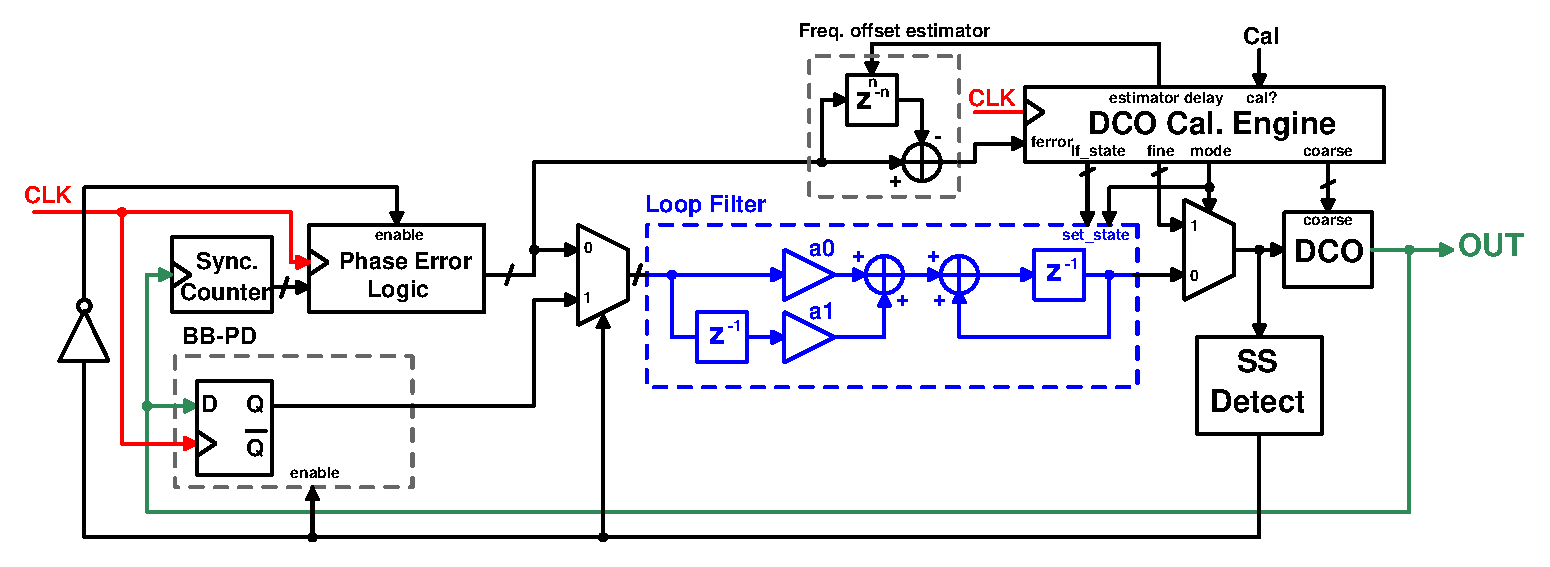
\includegraphics[width=0.8\textwidth, angle=0]{pll_master_arch_28feb2020}

	\end{block}
		\begin{block}{Power Targets {\color{red}(revised)}}
		\scriptsize
		{\color{red}\textbf{(Divider not necessary)}}
		\vspace{-1em}
		\begin{table}[htb!]
			\tiny
			\centering
			\def\arraystretch{1.5}		
			\setlength\arrayrulewidth{0.75pt}
			\setlength{\tabcolsep}{1em} % for the horizontal padding
			\begin{tabular}{|c|c|c|c|c|}
				\hline 
				\rule[-1ex]{0pt}{2.5ex} \cellcolor{gray!40}\textbf{DCO} & \cellcolor{gray!40}\textbf{Phase detector} & \cellcolor{gray!40}\textbf{Digital (LF)}& \cellcolor{gray!40}\textbf{Other} & \cellcolor{gray!40}\textbf{SUM} \\ 
				\hline 
				\rule[-1ex]{0pt}{2.5ex} 50 $\mu$W& 10 $\mu$W &  10 $\mu$W  & \textbf{0} {\color{red}\st{$\leq$ 5}} $ \mu$W & $\leq$ \textbf{70} {\color{red}\st{100}} $\mu$W\\ 
				\hline 
			\end{tabular} 
			% \caption{Assigned specifications for branch line hybrid design.}
			% \label{asgn_specs}
		\end{table}   
	\end{block}

\end{frame}

% #############################################################################
% Specification
% #############################################################################

\begin{frame}
	\frametitle{Specification\color{black}}
	\begin{block}{System Performance Targets}
		\tiny
		\begin{table}[h!]
			\centering
			\def\arraystretch{1.5}		
			\setlength\arrayrulewidth{0.75pt}
			\setlength{\tabcolsep}{1em} % for the horizontal padding
			\begin{tabular}{|l|r|l|l|}
				\hline 
				\rule[-1ex]{0pt}{2.5ex} \cellcolor{gray!40}\textbf{Parameter} & \cellcolor{gray!40}\textbf{Value} & \cellcolor{gray!40}\textbf{Unit }& \cellcolor{gray!40}\textbf{Notes}\\ 
				\hline 
				\rule[-1ex]{0pt}{2.5ex} \textbf{Frequency}  & 2.4-2.4835 & GHz & 2.4G ISM Band\\ 
				\hline 
				\rule[-1ex]{0pt}{2.5ex} \textbf{Ref. frequency} & 16 & MHz & Yields 6 channels \\ 
				\hline 
				\rule[-1ex]{0pt}{2.5ex} \textbf{Power} & $\leq$ \textbf{70} {\color{red}\st{75}} $\mu$W  &$\mu$W & Minimize!\\ 
				\hline 
				\rule[-1ex]{0pt}{2.5ex} \textbf{FSK BER} & $\leq$ 1e-2  & & GFSK\textbf{*} with $f_{dev}$=$\pm$250 KHz\\ 
				\hline 
				\rule[-1ex]{0pt}{2.5ex} \textbf{CNR} & $>$ 20 & dBc&Yields  \textbf{-235} dB FOM$_{jitter}$ ideally \\ 
				\hline 
				\rule[-1ex]{0pt}{2.5ex} \textbf{Initial Lock Time} & $\leq$ 10 & $\mu$s & Upon cold start \\ 
				\hline 
				\rule[-1ex]{0pt}{2.5ex} \textbf{Re-lock Time} & $\leq$ 5 & $\mu$s & Coming out of standby, $f_{error} <$ \textbf{1 MHz} \\ 
				\hline 
				\rule[-1ex]{0pt}{2.5ex} \textbf{Lock $\Delta f$ tolerance} & $100$ & kHz& \\ 
				\hline 
				\rule[-1ex]{0pt}{2.5ex} \textbf{FOM}$_{\textnormal{jitter}}$ & $\leq$ -230 & dB & \textbf{For state of art in size/power} \\ 
				\hline 
				\rule[-1ex]{0pt}{2.5ex} \textbf{Area} & $<$ 0.01  & mm$^2$ & \\ 
				\hline 
			\end{tabular} 
			% \caption{Assigned specifications for branch line hybrid design.}
			% \label{asgn_specs}
		\end{table}   
		\textbf{*} Using BT=0.3, 1 MSymbols/s, 4 demodulated symbols averaged per bit to yield 250 kbps.
	\end{block}    
\end{frame}



\begin{frame}
	\frametitle{Specification\color{black}}
	\begin{block}{Component-level specs}
		\scriptsize
	\begin{table}[h!]
		\centering
		\tiny
		\def\arraystretch{1.5}		
		\setlength\arrayrulewidth{0.75pt}
		\setlength{\tabcolsep}{1em} % for the horizontal padding
		\begin{tabular}{|l|r|l|}
			\hline 
			\rule[-1ex]{0pt}{2.5ex} \cellcolor{gray!40}\textbf{Parameter} & \cellcolor{gray!40}\textbf{Value} & \cellcolor{gray!40}\textbf{Unit }\\ 
			\hline 
			\rule[-1ex]{0pt}{2.5ex} \textbf{Counter range}  & 256 steps & coverage of 150-155 \\ 
			\hline 
			\rule[-1ex]{0pt}{2.5ex} \textbf{Divider ratio} & 150-155  & (For non-counter based)\\ 
			\hline 
			\rule[-1ex]{0pt}{2.5ex} {\color{red}\st{\textbf{TDC resolution}}} &{\color{red}\st{$\geq$ 155}}  & {\color{red}\st{steps/reference cycle}}\\ 
			\hline 
			\rule[-1ex]{0pt}{2.5ex} \textbf{DCO gain $K_{DCO}$} & $10^4$ & Hz/LSB \\ 
			\hline 
			\rule[-1ex]{0pt}{2.5ex} \textbf{DCO tuning range} & 10 & MHz \\ 
			\hline 
			\rule[-1ex]{0pt}{2.5ex} \textbf{DCO DAC resolution} & 10 & bit \\ 
			\hline 
			\rule[-1ex]{0pt}{2.5ex} \textbf{DCO Phase noise} &$<$ -80 & dBc/Hz @ $\Delta f=10^6$ Hz, $f_c$ = 2.448 GHz \\ 
			\hline 
			\rule[-1ex]{0pt}{2.5ex} \textbf{DCO Power} & $\leq$ 50 & $\mu$W \\ 
			\hline 
			\rule[-1ex]{0pt}{2.5ex} \textbf{Digital filter word resolution} & $\leq$ 16 & bits (power grows as $\mathcal{O}(n^2)$) \\ 
			\hline 
			\rule[-1ex]{0pt}{2.5ex} \textbf{BB-PD jitter} & $\leq$ 12 & ps$_{\textnormal{rms}}$ \\ 
			\hline 
		\end{tabular} 
		% \caption{Assigned specifications for branch line hybrid design.}
		% \label{asgn_specs}
		\label{design_specs}
	\end{table}   
	\end{block}    
\end{frame}

% #############################################################################
% Timeline
% #############################################################################

\begin{frame}
	\frametitle{Time plan (pt. 1)}
	\begin{table}[htb!]
		\tiny
		\centering
		\vspace{-1em}
		\def\arraystretch{1.5}		
		\setlength\arrayrulewidth{0.75pt}
		\setlength{\tabcolsep}{1em} % for the horizontal padding
		\begin{tabular}{|c|l|l|l|}
			\hline 
			\rule[-1ex]{0pt}{2.5ex}\cellcolor{gray!40}\textbf{Week \#} & \cellcolor{gray!40}\textbf{Dates} &\cellcolor{gray!40}\textbf{Tasks} & \cellcolor{gray!40}\textbf{Outcomes}\\ 
			\hline 
			% \rule[-1ex]{0pt}{2.5ex} \cellcolor{green!20}\textbf{3}&\cellcolor{green!20}13.1 - 19.1 &\cellcolor{green!20}Review PLL Design &\cellcolor{green!20}Refreshed Knowledge\\ 
			% \hline 
			\rule[-1ex]{0pt}{2.5ex}\cellcolor{red!40}\textbf{4}&\cellcolor{red!40}20.1 - 26.1 &\cellcolor{red!40}Finalize high level modeling &\cellcolor{red!40}Component level specification\\ 
			\hline 
			\rule[-1ex]{0pt}{2.5ex}\textbf{5}\cellcolor{red!40}&\cellcolor{red!40}27.1 - 2.2 &\cellcolor{red!40}Establish test bench in Virtuoso &\cellcolor{red!40}With ideal PLL implementation\\ 
			\hline 
			\rule[-1ex]{0pt}{2.5ex}\cellcolor{red!40}\textbf{6}&\cellcolor{red!40}3.2 - 9.2&\cellcolor{red!40}Schem. design: phase detector &\cellcolor{red!40}TDC - flash and counter based \\ 
			\hline 
			\rule[-1ex]{0pt}{2.5ex}\cellcolor{red!40}\textbf{7}&\cellcolor{red!40}10.2 - 16.2&\cellcolor{red!40}Schem. design: phase detector &\cellcolor{red!40}Bang-bang phase detector\\ 
			\hline 
			\rule[-1ex]{0pt}{2.5ex}\cellcolor{red!40}\textbf{8}&\cellcolor{red!40}17.2 - 23.2&\cellcolor{red!40}RTL, synthesis, place\&route &\cellcolor{red!40}Digital loop filter\\ 
			\hline 
			\rule[-1ex]{0pt}{2.5ex}\cellcolor{red!40}\textbf{9}&\cellcolor{red!40}24.2 - 1.3&\cellcolor{red!40}RTL, synthesis, place\&\cellcolor{red!40}route & \cellcolor{red!40}Digital loop filter\\ 
			\hline 
			\rule[-1ex]{0pt}{2.5ex}\cellcolor{green!40}\textbf{10}&\cellcolor{green!40}2.3 - 8.3&\cellcolor{green!40}Schem. design: oscillator &\cellcolor{green!40}Ring DCO\\ 
			\hline 
			\rule[-1ex]{0pt}{2.5ex}\textbf{11}&9.3 - 15.3& Layout: oscillator & \\ 
			\hline 
			\rule[-1ex]{0pt}{2.5ex}\textbf{12}&16.3 - 22.3& CDAC  & Schem+layout\\ 
			\hline 
			\rule[-1ex]{0pt}{2.5ex}\textbf{13}&23.3 - 29.3& Calibration& RTL/schem. for calibration\\ 
			\hline 
			\rule[-1ex]{0pt}{2.5ex}\textbf{14}& 30.3 - 5.4 &  Flex week - schem. design & Finalize schematic level design\\ 
			\hline 
			\rule[-1ex]{0pt}{2.5ex}\textbf{15}& 6.4 - 12.4& {\color{red}\textbf{Easter}} & - \\ 
			\hline 
			\rule[-1ex]{0pt}{2.5ex}\textbf{16}& 13.4 - 19.4& Layout & Phase detector\\ 
			\hline 
			\rule[-1ex]{0pt}{2.5ex}\textbf{17}& 20.4 - 26.4& Layout & Oscillator\\ 
			\hline 
		\end{tabular}
		\begin{flushleft}\textbf{Legend:} \colorbox{red!20}{\textbf{Done}} \colorbox{green!20}{\textbf{Current}}  \colorbox{blue!20}{\textbf{Revised}}
		% *I will write the report simultaneously with the work.
		\end{flushleft}
		% \caption{Assigned specifications for branch line hybrid design.}
		% \label{asgn_specs}
	\end{table}   
\end{frame}

\begin{frame}
	\frametitle{Time plan (pt. 2)}
	\begin{table}[htb!]
		\tiny
		\centering
		\vspace{-1em}
		\def\arraystretch{1.5}		
		\setlength\arrayrulewidth{0.75pt}
		\setlength{\tabcolsep}{1em} % for the horizontal padding
		\begin{tabular}{|c|l|l|l|}
			\hline 
			\rule[-1ex]{0pt}{2.5ex}\cellcolor{gray!40}\textbf{Week \#} & \cellcolor{gray!40}\textbf{Dates} &\cellcolor{gray!40}\textbf{Tasks} & \cellcolor{gray!40}\textbf{Outcomes}\\ 
			\hline 
			\rule[-1ex]{0pt}{2.5ex}\textbf{18}& 27.4 - 3.5 & Layout & Divider/calibration\\ 
			\hline 
			\rule[-1ex]{0pt}{2.5ex}\textbf{19}& 4.5 - 10.5 & Layout & Finalization/system integration\\ 
			\hline 
			\rule[-1ex]{0pt}{2.5ex}\textbf{20}& 11.5 - 17.5 & Flex week (layout) OR yield improvement & Depending on progress\\ 
			\hline 
			\rule[-1ex]{0pt}{2.5ex}\textbf{21}& 18.5 - 24.5& {\color{blue}\textbf{Report writing}} & \\ 
			\hline 
			\rule[-1ex]{0pt}{2.5ex}\textbf{22}& 25.5 - 31.5& {\color{blue}\textbf{Report writing}} & \\ 
			\hline 
			\rule[-1ex]{0pt}{2.5ex}\textbf{23}& 1.6 - 7.6& {\color{blue}\textbf{Report writing}} & {\color{red}\textbf{Deadline 8.6}}\\ 
			\hline 
		\end{tabular}
		\begin{flushleft}\textbf{Legend:} \colorbox{red!20}{\textbf{Done}} \colorbox{green!20}{\textbf{Current}}  \colorbox{blue!20}{\textbf{Revised}}
		% *I will write the report simultaneously with the work.
		\end{flushleft}
		% \caption{Assigned specifications for branch line hybrid design.}
		% \label{asgn_specs}
	\end{table}   
\end{frame}


% #############################################################################
% project phases
% #############################################################################

% ############################################################################b#
% References
% #############################################################################


\begin{frame}
	\frametitle{References}
		\scriptsize
		[1] L. Dai and R. Harjani, "Analysis and design of low-phase-noise ring oscillators," ISLPED'00: Proceedings of the 2000 International Symposium on Low Power Electronics and Design (Cat. No.00TH8514), Rapallo, Italy, 2000, pp. 289-294. doi: 10.1145/344166.344639\par
		\vspace{0.5em}
		[2] A. Hajimiri and T. H. Lee, "A general theory of phase noise in electrical oscillators," in IEEE Journal of Solid-State Circuits, vol. 33, no. 2, pp. 179-194, Feb. 1998.\par
		% [1]  Liu, H., Shirane, A., Okada, K., Sun, Z., Huang, H., Deng, W., Siriburanon, T., Pang, J., Wang, Y., Wu, R. and Someya, T. (2019). A 265-$\mu$ W Fractional-${N}$ Digital PLL With Seamless Automatic Switching Sub-Sampling/Sampling Feedback Path and Duty-Cycled Frequency-Locked Loop in 65-nm CMOS. IEEE Journal of Solid-State Circuits, 54(12), pp.3478-3492.
		\vspace{0.5em}
		[3] G. Jacquemod et al., "Study and reduction of variability in 28 nm FDSOI technology," 2015 International Workshop on CMOS Variability (VARI), Salvador, 2015, pp. 19-22.\par
		\vspace{0.5em}

		% [1]  H. Xu and A. A. Abidi, “Design Methodology for Phase-Locked Loops Using Binary (Bang-Bang) Phase Detectors,” IEEE Transactions on Circuits and Systems I: Regular Papers, vol. 64, no. 7, pp. 1637–1650, Jul. 2017.\par
		% \vspace{0.5em}
		% [2] F. Gardner, “Charge-Pump Phase-Lock Loops,” IEEE Transactions on Communications, vol. 28, no. 11, pp. 1849–1858, Nov. 1980, doi: 10.1109/tcom.1980.1094619.\par
		% \vspace{0.5em}
		% [3] Liu, B., Li, Z., Fu, X., Shirane, A., Kurosu, H., Nakane, Y., Masaki, S., Okada, K., Zhang, Y., Qiu, J., Huang, H., Sun, Z., Xu, D., Zhang, H., Wang, Y. and Pang, J. (2020). A Fully-Synthesizable Fractional-N Injection-Locked PLL for Digital Clocking with Triangle/Sawtooth Spread-Spectrum Modulation Capability in 5 nm CMOS. IEEE Solid-State Circuits Letters, pp.1-1.
	% Navid et al. 2005
\end{frame}


\end{document}
